\chapter{Design Principles for Energy--Efficient Applications}
\label{chapter:energydesignprinciples}

\section{Introduction}

Digital-transformation initiatives have led to major efficiencies and cost savings, including the transition from paper-based processing to electronic documents and the use of traffic-routing algorithms for vehicle navigation. However, the software performing this new computerised work consumes nearly 10 percent of the world's electricity \cite{mills2013-digital-energyusage}. Today's cloud-based applications span multiple continents, consuming energy in servers, networks, cooling and power facilities, storage, and user devices.

As discussed in \sref{sec:litreviewenergy}, over the past decade researchers have been studying IT infrastructure energy consumption, working to increase datacenter, network, and hardware efficiency. A number of significant research projects (such as DC4Cities \cite{dc4cities2014_dcmetrics} and the European Commission's work on data centre efficiency \cite{eu2018-datacentreenergy}) have brought promising research together with interested practitioners in order to find practical solutions to the problem of ever-increasing energy consumption for the world's ongoing digital transformation.  As a result, datacenter energy efficiency has improved considerably. For example, in the US, public-sector datacenters now often operate at a power usage effectiveness (PUE) of less than 1.5, whereas a PUE of 2 was considered normal only a few years ago. \footnote{PUE is a datacenter's total energy consumption divided by its IT energy consumption, usually measured over one year. A PUE of 1.5 indicates that for every 1 KWh of IT load, a datacenter requires an additional 0.5 KWh.}

Individual hardware devices have experienced a similar trend and computations per joule of energy have doubled roughly ever 18 months over the past two decades \cite{koomey2011-trends-energy-efficiency}. 

However an aspect of energy efficiency that has been largely neglected is the efficiency of the software applications underpinning this digital revolution, and specifically how to provide the software architecture practitioners designing them with practical guidance on how to take energy properties into account as they design their systems.  In this chapter we start to address this situation and present three simple design principles that software architects can use to address system-level energy efficiency. We also present a case study that inspired the creation of the principles and illustrates the energy savings possible with a holistic architecture-led approach.

\section{The Challenge for Software Architects}

We suspected that software architects might find it difficult to prioritize energy efficiency for three main reasons. 

First, we have little practical understanding of how design decisions affect energy efficiency or other system qualities such as user experience, reliability, and performance. Without this knowledge, analyzing tradeoffs to elucidate the benefits or costs of improving energy efficiency is difficult.

Second, to achieve meaningful improvements in energy efficiency, architects must gain new technical knowledge beyond traditional design boundaries. This will require that people from different specializations and departments work together. Such collaboration is challenging given the structure of many organizations that inadvertently prevent such collaboration through competing objectives, human dynamics and organisational barriers.

Finally, system acquirers and users rarely list energy efficiency as a major concern. This is partly because of split incentives. System operators such as administrators or datacenter managers don't pay for the energy bill directly - the budget for energy tends to be included in a separate facilities budget owned by a different manager. This means that they would see little or no direct personal benefit from any energy savings that they achieve.

A previous survey attempted to understand architects' perspectives on energy efficiency \cite{bashroush2016-datacentreenergy} and surveyed 12 representative, experienced architects from various organization types. They were asked whether they had encountered energy efficiency as an architectural concern in the previous five years and whether they believed that they had the right tools to address energy related challenges. The survey also asked whether the participants believed that energy would be an important architectural concern over the next five years.

The survey, while small, did include participants from a number of relevant sectors including 7 from technology consultancies, 1 from an Internet company, 2 from banking and finance and 2 from other industries.  Of these respondents, most of them (83\%) hadn't had to deal explicitly with energy concerns during the previous 5 years although interestingly 66\% of them thought that energy was an important concern that they would need do deal with over the next 5 years.  Given the state of the art, predictably, only 25\% of the respondents thought that they had the right tools to deal with energy as an architectural concern.  These findings are consistent with our industrial experience, where energy is rarely discussed as an architectural concern, when it is discussed it is usually seen as a hardware and data centre concern, and when application architects are concerned with it, they lack the methods and tools to allow them to understand and compare the energy implications of their architectural decisions.

\section{State of the Art}

To increase efficiency, we must be able to measure it. That is, we must be able to measure the useful work our software applications produce and the amount of energy this takes and then optimize the ratio between the two. However, although the datacenter world has metrics such as PUE, no comparable, generally agreed, metrics exist for software.

Optimization must also consider key quality properties such as resilience (because redundancy in system designs is usually a major contributor to energy consumption), usability, and performance. However architecture practitioners don't generally have access to such tools and techniques today \cite{bashroush2016-datacentreenergy}.

Despite these challenges, energy efficiency has been gaining traction in software engineering. Much of the early research focused on measuring applications' energy consumption \cite{islam2016-energysoftwarefeatures} and tried to define useful work so as to allow the creation of useful metrics (for example, the DC4Cities project we mentioned earlier \cite{dc4cities2014_dcmetrics}). In parallel, other researchers have explored compiler optimization to decrease energy consumption or have evaluated design patterns' energy efficiency.

All these efforts have helped us begin to understand and optimize software applications. However, improving today's Internet-scale systems will require a more wholistic approach that considers the whole system. Software architects are well placed to lead such an approach.

\section{The Three Principles}

On the basis of early industrial experience in successful projects to reduce energy consumption we propose three simple architecture principles for achieving energy-efficient systems:

\begin{itemize}
\item \emph{Principle 1}. Energy efficiency metrics must relate business transactions to energy consumption in a meaningful way to key system stakeholders.
\item \emph{Principle 2}. Identifying sources of energy waste at the system level produces the biggest savings.
\item \emph{Principle 3}. Addressing the energy optimization problem requires a \\ cross-disciplinary team.
\end{itemize}

These principles are discussed in more detail in the following subsections. 

\subsection{Relating Business Transactions to Energy Consumption}

Architectural priorities are set by the system's stakeholders, who the architects interact with to understand their needs and goals, trading these off to reach an acceptable set of architectural properties for the combined stakeholder group \cite{rozanski2011-ssa2e}.  In order for energy to be viewed as an important system quality, it must be explained, measured and its impact assessed in a way that significant system stakeholders can understand and relate to their own goals.  Ultimately, identifying suitable metrics and relating them to stakeholder goals can help to achieve a holistic approach to system quality property tradeoffs and hence drive revenue and cost optimization.

Like many other quality properties, we have observed that energy properties tend to be viewed as a purely technical concern, only of interest to stakeholders involved in system operation.  This means that today energy properties rarely become a concern of senior business stakeholders and so often do not have sufficient executive sponsorship to gain significant attention, when in competition with core concerns like functional coverage, performance or scalability.  Until recently we have also seen this effect in regards to security, which only recently has started to be a concern of key decision makers \cite{cisco2016-uksecprioritisation}.

The key to achieving alignment with the goals of senior decision makers is to relate energy characteristics of the system to the operational cost of the system and hence to characterise energy usage as part of the cost of executing business transactions.  The cost of a business transaction is quite simply the reduction in margin (profit) on that transaction and for many businesses, operating on slim single digit percentage margins, small improvements in per-transaction costs are attractive targets for engineering effort, as they return more and more benefit as the volume of business increases.

Of course, executive decision makers are only one type of stakeholder and an important part of the architect's job is to make the right tradeoff between the needs of different types of stakeholder.  The executive decision makers are normally the \emph{acquirers} of systems, being the budget holder and so operational cost and development cost are significant concerns for them.  Most systems have one or more type of \emph{assessor} in the compliance, audit, security or quality management groups.  The assessors are often interested in energy consumption from an environmental management compliance perspective.  While not directly a financial concern, compliance or audit assessors may well have environmental impact or direct energy efficiency goals that they are interested in achieving.  The \emph{systems administration} stakeholders encompass all those involved in operating system system (from data centre managers to individual administrators) and this group are often goaled with reducing their overall site (data centre) energy consumption and so will be motivated to work with application architects who are energy aware and can help to achieve application level reductions to contribute towards this goal.  The \emph{developers} of the software often aren't aware of their contribution towards a system's energy characteristics and can be difficult to motivate to priortise energy concerns unless there is a direct impact on user experience (such as IoT device software or mobile application developers who often have to be very aware of energy consumption to avoid exhausting battery based power sources).  This means that we are quite dependent on the \emph{architects} (who are themselves stakeholders in the application) to understand the wider context for application energy concerns and translate these into comprehensible goals for developers to incorporate into their work.

While different stakeholders have different perspectives on the energy properties of an application, in reality energy can affect an organisational in a number of ways including ethical (how to minimise the resources required to run the organisation), environmental (how to reduce or "green" energy consumption to reduce the organsiation's environmental impact), reputational (to avoid negative associations with careless use of natural resources or creation of pollution), cost (where reducing energy consumption will make a business more efficient) and agility (where energy efficiency can reduce the need to increase an organisation's physical data centre footprint in order to change or expand the organisation's business).  As more and more enterprises move to public cloud environments \cite{idc2016-cloudreport} these organisations need to focus on the direct ethical and reputational impacts of application energy consumption, and work with their cloud providers to address environmental and cost impact of their energy consumption (the cloud providers largely hide the possible impact on agility due to their huge scale). 

In summary, if the energy characteristics of an application are considered simply as an organisational level cost concern (as, for example, environmental emissions were a few years ago) then it is unlikely that they will ever get the attention required for architects to prioritise them as an architectural concern.  The role of application architects is to make the broad organisational impact clear and this involves transparency of usage, impact and cost for the different parts of the organisation that can have an effect on energy consumption.  Hence the architect needs to translate the technical energy metrics for different stakeholder groups to relate them to their goals in order to illustrate their impact on these goals and motivate different stakeholder groups to address energy concerns in a cross-organisational way. 

\subsection{Energy as a System Level Concern}

The second principle we have identified is that energy needs to be seen as a system level concern, and so be addressed at the application architecture level.  However our experience and review of the research literature suggests that many of the most practical existing approaches to dealing with energy efficiency and usage are at a micro level, measuring the energy usage of individual code procedures, or at the large scale macro level, analysing the energy usage of an entire data centre.  

While valuable in different situations, the problem is that neither the micro or macro view is useful when trying to understand and improve the energy efficiency of mainstream software applications.  If we measure energy efficiency at the level of individual code blocks, this is too fine-grained a level of detail for an application architect to use at any scale.  Improving measurements taken at this level can rarely have a big impact on system energy consumption as dozens or hundreds of such micro-level components combine to process a particular system usage scenario and it is very difficult to see which of the micro-level improvements have the biggest impact at system level.  On the other hand, the data-centre level level measurements, while useful for understanding the energy characteristics of the entire IT estate, also don't help the application architect, as the only metrics available are maximums, minimums and averages on sections of the infrastructure estate and these measurements do not allow an application architect to understand the energy implications of their architectural decisions.

It seems clear then that the most effective level of abstraction at which to consider application energy efficiency is at the architectural level of the application itself.  This allows us to consider the application as a complete system and to analyse usage patterns (scenarios) rather than individual components.  Scenarios describe how systems are used and so understanding their energy characteristics reveals the real runtime energy characteristics of an application.  Once a system's key usage scenarios are understood, then their energy characteristics can be analysed and the architect can use this information to allow the architect to see where to focus their effort for the most impact and the effect of their architectural descisions.

An example of how considering energy at an application level can help to focus effort where it will be the most effective is to consider how redundancy is used within an application.  Many applications use redundancy of system elements in order to achieve qualities like scalabilty and resilience.  However redundancy is a commonly overlooked source of energy consumption as it is often applied at all levels, including facilities, hardware, and software, due to the application not being considered as a wholistic system.   A system-level evaluation of resilience requirements allows the architect to identify where redundancy is unnecessary, which is a huge opportunity to achieve energy savings that would be difficult with local optimizations.

\subsection{Employing Cross-Disciplinary Teams}

Energy optimization requires design work across traditional design boundaries. For example, optimizing the design of resilience requires collaboration among infrastructure engineering, application development, and business teams. Without a collaborative approach, improvements will be restricted to local optimizations, which often miss the bigger opportunities for savings.

This problem is related to the problem of most energy efficiency work being performed at the micro (code block) or macro (data centre) level, as we described above.  These may be considered to be vertically separated areas of focus.  For this principle however we are concerned with the tendency for organisations to partition work between "horizontal" organisational groups, from the business organisation, through the application delivery teams, through the operational teams, to the data centre infrastructure organisation at the end.  This organisational separation of people and work encourages a tendency to believe that energy consumption is "someone else's problem".  For example, production operations groups view it as a problem with inefficient applications, whereas application development groups view it as a problem both with the lack of focus on energy by their business stakeholders and the "arbitary overheads" they believe are imposed by the production environment that their application runs within.

This organisational fragmentation can have many negative effects, but it is particularly serious when we are trying to address energy consumption concerns, as it results in the information needed to address energy concerns being scattered across organisational boundaries.  It is common to find hardware energy consumption metrics in one place, operating system counters in another, application tracing and monitoring somewhere else again, and data centre efficiency and overheads being yet another group.

The knowledge and skills needed to understand and address energy concerns also tend to be found in different teams, separated by organisational boundaries, as does the authority needed to make meaningful change and effectively evaluate the impact of a change, as this will be at multiple levels of abstraction and ranges of authority.

All of these factors mean that for us to address energy concerns effectively, we need organisations to form cross-functional teams to take shared accountability for driving down energy usage by finding the most effective places to focus their attention, identify solutions to those problems, and then to gain the consensus and commitment to addressing them.

\section{Case Study: Online Auction Site}

The energy management principles we identified above were inspired by the work performed by architects at eBay, the Internet auction site, who identified a number of significant architectural design decisions to improve energy efficiency and from which we identified these principles.

In order to reduce its environmental impact, while also reducing cost, eBay introduced a programme known as the Digital Service Efficiency (DSE) initiative \cite{ebay2013-digitalefficiency} which aimed to increase the efficiency of the eBay platform. DSE relates business metrics such as volumes and value of customer transactions to their energy consumption and environmental impact.   The approach they defined designed a set of metrics that were meaningful to key stakeholders across the business, which helped the organisation to understand, analyse and reduce its energy consumption, while understanding the architectural tradeoffs that this involved (which is the basis of Principle 1). Some of the metrics that the DSE programme defined were the number of buy transactions per kWh of energy consumed, the number of sell transactions per kWh of energy consumed, the revenue generated per MW of power consumed, and the volume of CO2 emissions per million active eBay users.

The organisation identified that reducing infrastructure redundancy was as one of its key opportunities to save energy at an acceptable level of cost and effort. In order to achieve this, eBay considered energy consumption at a system architecture level and made significant architectural changes that would result in large improvements in energy efficiency.  They achieved this by reconsidering the assumptions and tradeoffs between business requirements for resilience and the cost of introducing redundancy in the architecture (this was the basis of Principle 2).  The key architectural insight that allowed them to make this step was the realisation that no matter how resilient its data-centre application services were, if the client application (a mobile app or web browser application) failed then the whole session failed and the client applications failed a lot more frequently than the data-centre services.  Through their analysis they came to realise that in many cases, making the data-centre application services more resilient would not increase resilience as experienced by their end users and so a high degree of redundancy in the data-centre services was unnecessary in many cases. This meant that responsibility for system resilience could be moved to the weakest link: the client application (i.e. the eBay web user interface and the eBay mobile applications).

To capitalise on this opportunity, they defined a new achitectural pattern for client access to application services and introduced a service request proxy component in the client applications. The client applications call the proxy, rather than the services, and the role of the proxy is to implement a timeout feature so that when a service request has exceeded a reasonable period of time, the proxy will automatically reissue the request, which will be routed to another service instance.  Hence if a service fails during a client's service request then the client is unaware of this provided that the proxy's duplicate request can be routed to another surviving service instance.  While not necessarily suitable for transactional services (like payments) due to complications with idempotency, this approach works very well for non-transactional or less-critical services like search requests or user profile updates.  This allows the non-critical or non-transactional services to be significantly simplified and data-centre side redundancy and retry to be eliminated because the proxy's operation can mask their failures.

Using their existing business analytics, eBay estimated that only about 10 percent of service requests needed to be considered as critical transactions, such as payments (which has specific regulatory needs and is normally expected to be executed on a highly available infrastructure). This insight allowed eBay to process critical transactions at a separate, smaller, highly resilient datacenter that has a fraction of the capacity of the main datacenters \cite{nelson2013-ebaycasestudy} while processing most of the service invocation workload using a cheaper, less resilient infrastructure. This provided a significant improvement in energy efficiency and required collaborative work across eBay's engineering, operational, and business teams (which led to Principle 3).

Figure \ref{figure:styles} depicts eBay's original and new more energy-efficient architectures. The new architecture allows for reduced datacenter redundancy while maintaining overall system performance and resilience.

\begin{figure}
\centering
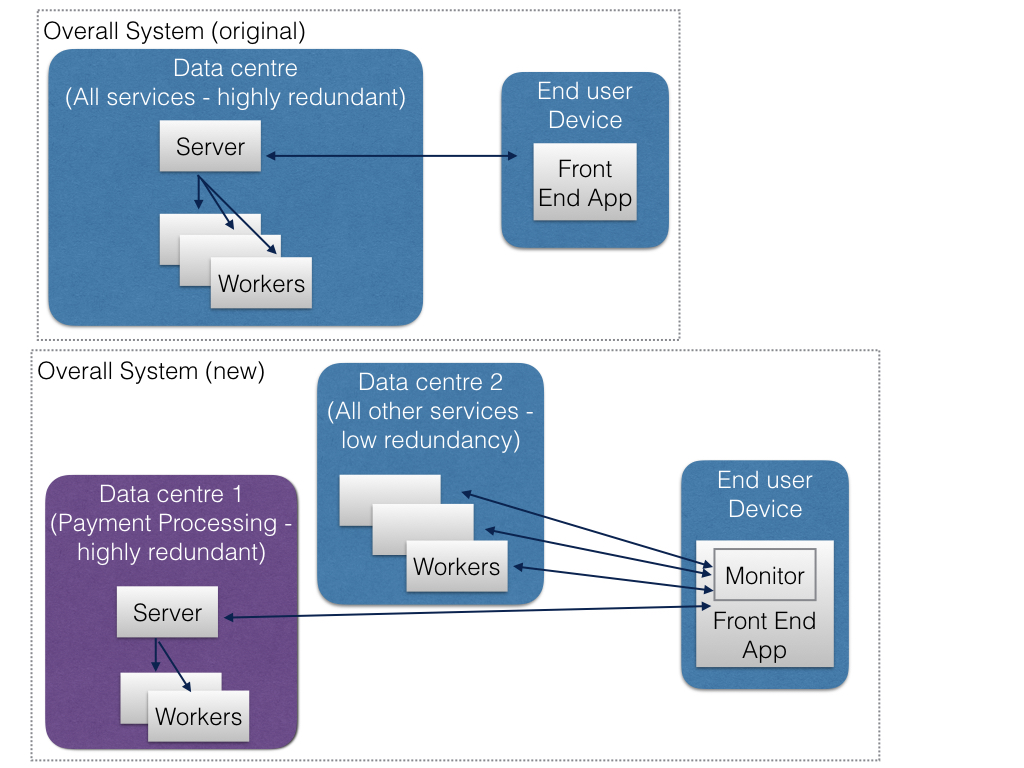
\includegraphics[width=\textwidth]{Figures/principles-styles}
\caption{eBay's Architectural Evolution for Energy Efficiency}
\label{figure:styles}
\end{figure}

This new architecture allowed eBay to achieve major capital and operational expenditure savings and well as reducing their energy consumption significantly. This was due to the simpler design of the low-redundancy services, which have substantially decreased the amount and complexity of infrastructure needed.  As a consequence, they have achieved a significant reduction in datacenter build-out and fit-out costs and time scales. The underlying factor that allowed this improvement was that redundancy costs are significant. For example, according to Steven Shapiro, the cost of building a Tier III datacenter is double that of a Tier II datacenter \cite{shapiro2015-datacentre-mythsrealities}. (The Tier Classification System is a widely used rating system for datacenter availability, with Tier I being the least available or redundant facility and Tier IV the highest \cite{uptime2015-tierclassification}.)

Even more important (from our perspective), eBay has reduced energy consumption by approximately 50 percent because the low-redundancy site requires fewer infrastructure components (for example, N + 1 rather than 2N + 1 redundancy). This has resulted in  significant energy cost savings and also a reduction in maintenance and hardware refresh requirements, further lowering environmental costs.

\section{Conclusions}

There has been increased interest in reducing the significant energy costs of running large IT systems. However, little attention has been given to addresing energy efficiency at an application level, which prevents software architects from considering energy as a first class architectural concern.  When software architects do attempt to understand the energy property implications of their decisions, they find that they lack suitable tools and methods to address energy concerns when designing systems. With this challenge in mind, we've investigated how a large organisation solved this challenge and from that experience suggested three practical principles to guide architectural decision making, which architects can use to guide energy-related tradeoffs during system design even with today's limited knowledge and technology.

Despite these principles' simplicity, the eBay experience shows that they can yield significant cost and energy savings when applied to large-scale production systems. Savings of this scale are difficult to achieve through local optimizations, so we must address the problem at a system level, and ensure we allow software architects to work across stakeholder groups and organisational boundaries in order to achieve meaningful results.
